\section{Resultados}

Conociendo los valores iniciales de la se\~nal limpia, el ruido proporcionado y
habiendo obtenido el resultado luego de aplicar los filtros, resulta muy
sencilla una primera aproximaci\'on a los resultados. La idea del experimento es
intentar que la se\~nal recuperada se parezca lo m\'as posible a la original
(sin ruido).

Fue simple entonces observar la diferencia entre la se\~nal recuperada y
la original de manera gr\'afica, ya sea a trav\'es de ploteos de se\~nales de 1
\'o 2 dimensiones como de la fuente misma como son las im\'agenes en 2
dimensiones.

Acompa\~nando esto por m\'etodos anal\'iticos como el PSNR (Relaci\'on Se\~nal a
Ruido de Pico) fue posible analizar que filtros resultan mejores que otros y en
que casos es mejor aplicar cada uno.

\subsection{Primeros resultados}

Experimentalmente pudimos observar que el filtro cero es bueno (recupera las
se\~nales en un grado aceptable), pero el filtro 
exponencial y el de la mediana son bastante mejores en general. En el caso
de ruido Impulsivo, el filtro de la mediana logra resultados interesantes.

Para poder obtener un mejor filtrado del ruido, decidimos aplicar primero el 
filtro exponencial y luego el de la mediana, lo que result\'o en un filtrado muy 
interesante, dando buenos resultados en ciertos casos. 

Los adjetivos utilizados se apoyan tanto en la interpretaci\'on de los gr\'aficos,
la apreciaci\'on del resultado en las im\'agenes y la medida del PSNR tanto en 1 como en 2
dimensiones. 

\subsection{Se\~nales en una dimensi\'on}

\subsubsection{Filtro Cero}

El primer filtro analizado fue el m\'as sencillo de implementar, el filtro cero.
Como mencionamos anteriormente, este filtro utiliza un umbral y env\'ia los
puntos que lo sobrepasan (tanto por arriba como por debajo) a cero.

\begin{figure}[H]
\begin {center}
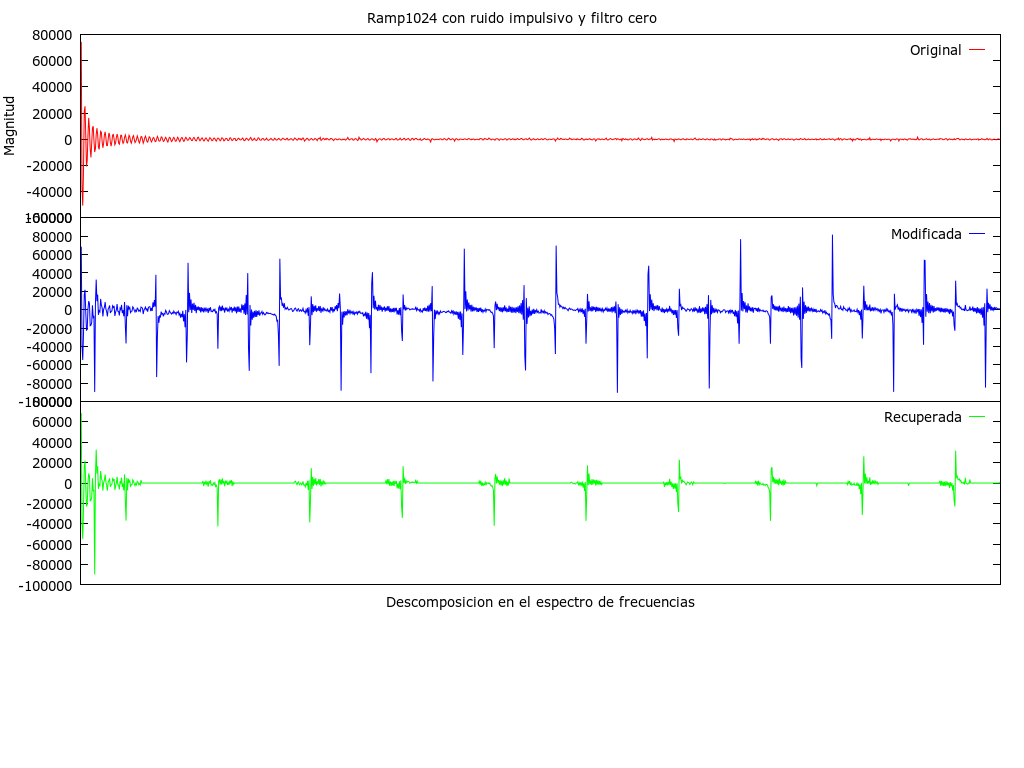
\includegraphics[width=500pt]{imagenes/ramp1234-imp-zero.png}
\end {center}
\caption{Se\~nal \texttt{ramp1234} provista por la c\'atedra, en el dominio de frecuencias, gr\'aficada
luego de aplicar ruido impulsivo (azul) y habiendo aplicado el filtro cero (verde)}
\label{fig:Dopp1024zero}
\end{figure}


\subsubsection{Filtro Exponencial}



\begin{figure}[H]
\begin {center}
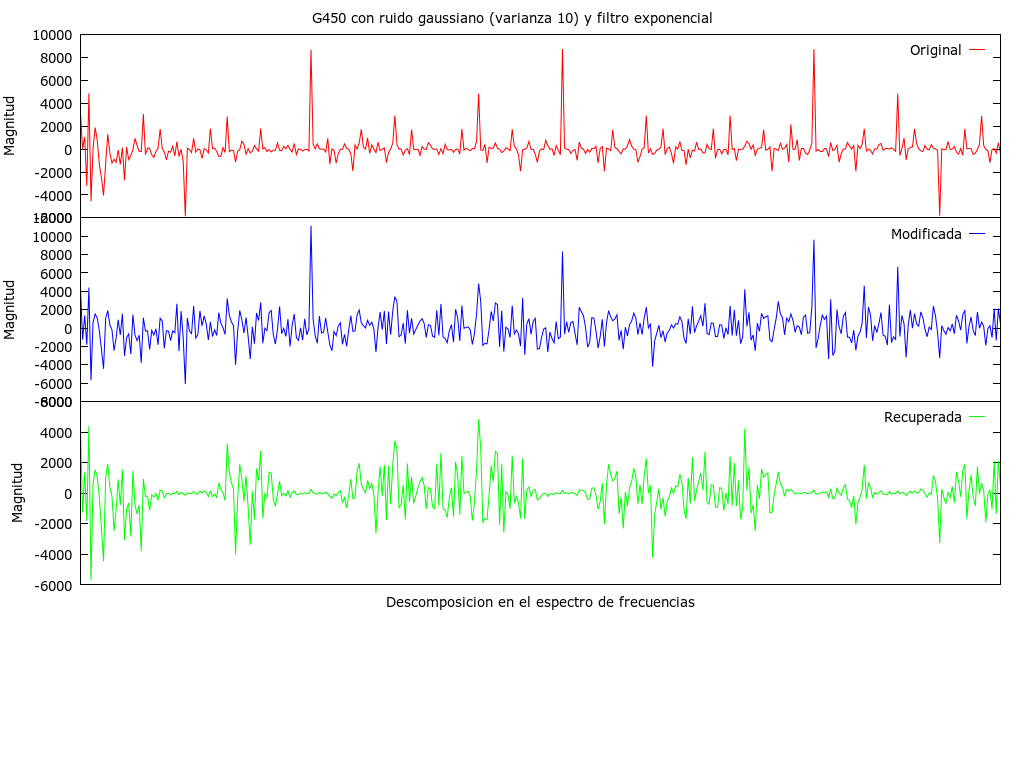
\includegraphics[width=500pt]{imagenes/g450-gauss-10-exp.png}
\end {center}
\caption{Se\~nal \texttt{g450} provista por la c\'atedra, en el domino de frecuencias, gr\'aficada
luego de aplicar ruido gaussiano con varianza 10 (rojo) y 
habiendo aplicado el filtro exponencial (azul)}
\label{fig:GexpSpec}
\end{figure}

\begin{figure}[H]
\begin {center}
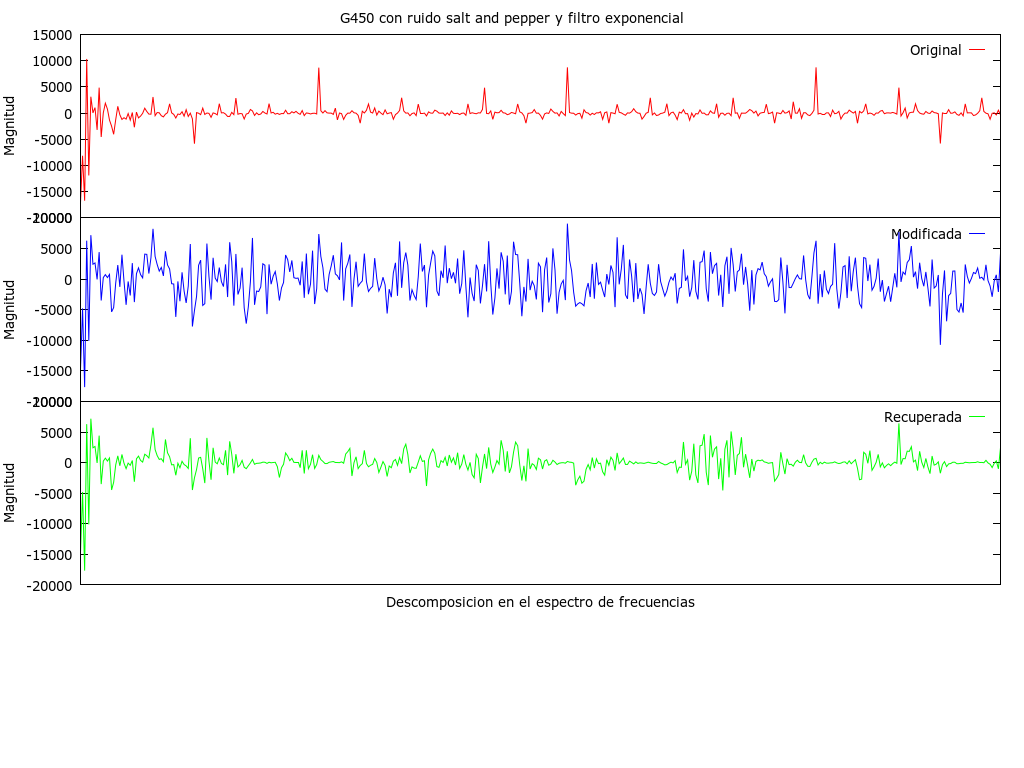
\includegraphics[width=500pt]{imagenes/g450-imp-exp.png}
\end {center}
\caption{Se\~nal \texttt{g450} provista por la c\'atedra, en el domino de frecuencias, gr\'aficada
luego de aplicar ruido impulsivo (azul) y habiendo aplicado el filtro exponencial (verde)}
\label{fig:SexpSig}
\end{figure}

\subsubsection{Filtro de la Mediana}

\begin{figure}[H]
\begin {center}
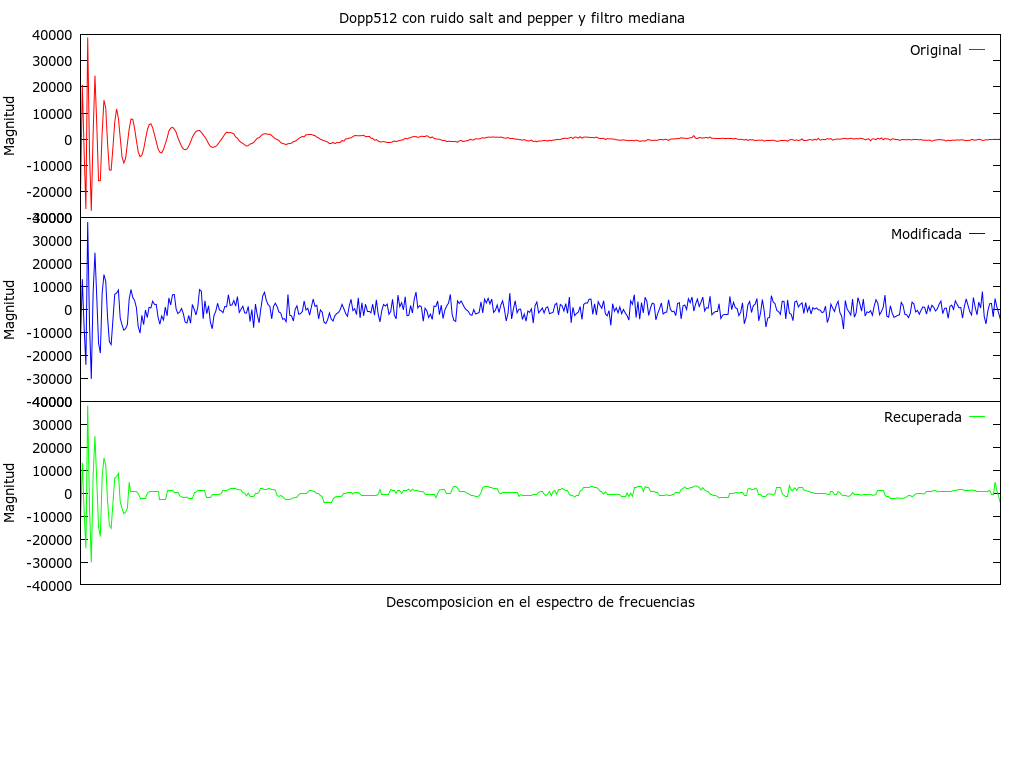
\includegraphics[width=500pt]{imagenes/dopp512-imp-median.png}
\end {center}
\caption{Se\~nal \texttt{doppler512} provista por la c\'atedra, en el dominio de frecuencias, gr\'aficada
luego de aplicar ruido impulsivo (azul) y habiendo aplicado el filtro de la mediana (verde)}
\label{fig:SinProm}
\end{figure}


\subsubsection{M\'ultiples filtros}

\begin{figure}[H]
\begin {center}
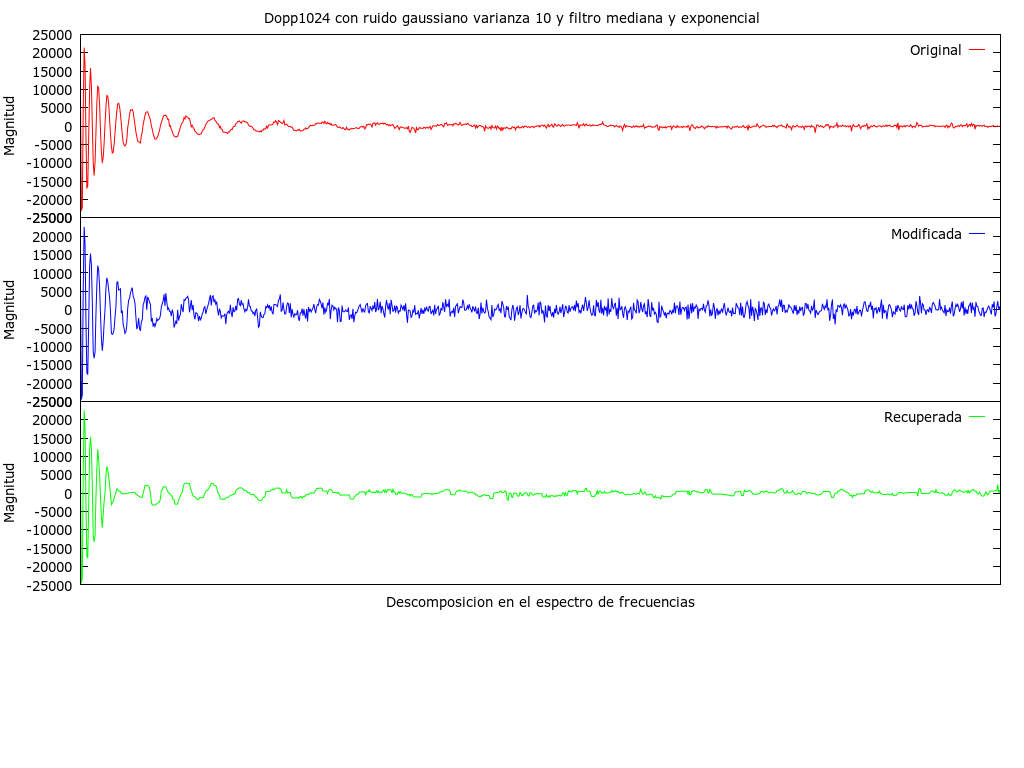
\includegraphics[width=500pt]{imagenes/dopp1024-gauss-10-both.png}
\end {center}
\caption{Se\~nal \texttt{doppler1024} provista por la c\'atedra, en el dominio de frecuencias, gr\'aficada
    luego de aplicar ruido gaussiano de varianza 10 (azul) y 
habiendo aplicado los filtros de la mediana y exponencial (en ese orden) (verde)}
\label{fig:gcomb}
\end{figure}

\begin{figure}[H]
\begin {center}
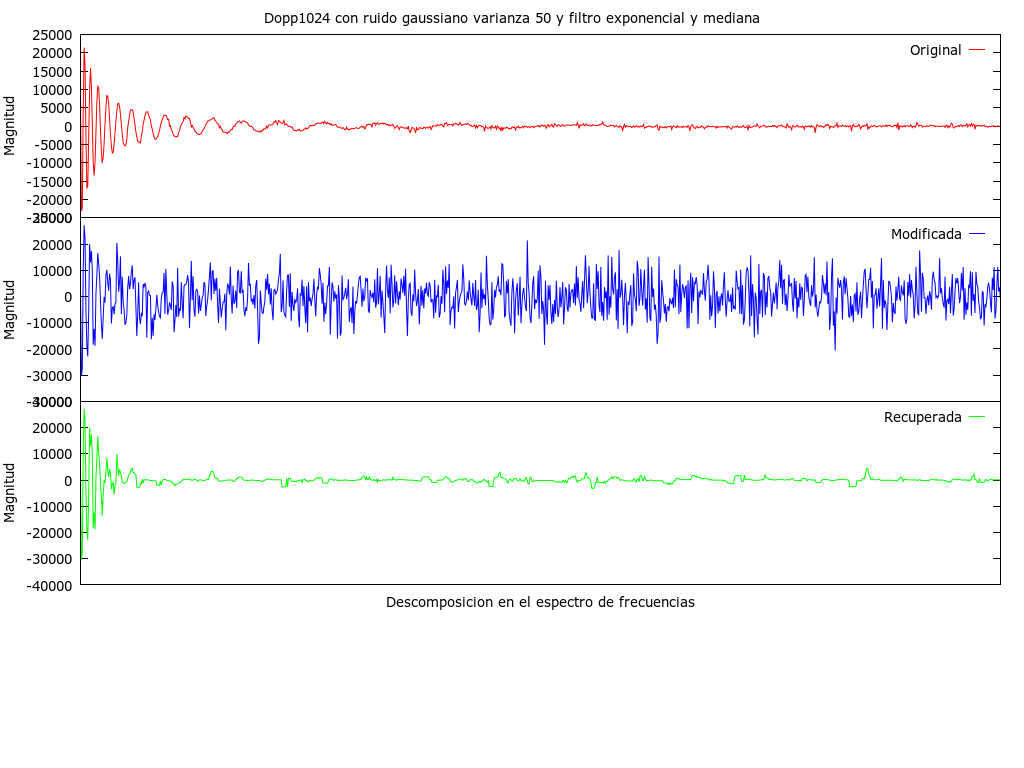
\includegraphics[width=500pt]{imagenes/dopp1024-gauss-50-bothr.png}
\end {center}
\caption{Se\~nal \texttt{doppler1024} provista por la c\'atedra, en el dominio de frecuencias, gr\'aficada
luego de aplicar ruido gaussiano utilizando una varianza de 50 (azul) y 
habiendo aplicado los filtros exponencial y de la mediana (en ese orden) (verde)}
\label{fig:dopcomb}
\end{figure}

\newpage
\subsection{PNSR de 1D}

\subsubsection{Tabla de resultados para ruido blanco de varianza 10}

\begin{table}[H]
        \begin{tabular}{|l|lllll|}
                \hline
                \textbf{PSNR [dB]} & Se\~nal + Gaussian (0,10) & F(Zero) & F(Exp) & F(Mediana) & F(Ambos) \\ \hline
                    Dopp512 & 11.6843 & 12.8369 & 15.3068 & 12.9666  \\
                    Dopp1024 & 13.0023 & 14.0229 & 19.7479 & 17.2167  \\
                    s64 & 8.12886 & 8.39132 & 14.0562 & 8.24892 \\
                    Ramp1234 & 28.0286 & 27.593 & 25.8266 & 27.8568  \\
                    g450 & 24.7025 & 24.7641 & 25.0357 & 25.4474  \\ \hline
                    \end{tabular}
                \end{table}


\subsubsection{Tabla de resultados para ruido blanco de varianza 50}

\begin{table}[H]
        \begin{tabular}{|l|lllll|}
                \hline
                \textbf{PSNR [dB]} & Se\~nal + Gaussian (0,50) & F(Zero) & F(Exp) & F(Mediana) & F(Ambos) \\ \hline
                    Dopp512 & 7.99957 & 0.642589 & 0.660194 & 6.63712 \\
                    Dopp1024 & 15.5627 & 1.41572 & 1.19794 & 8.00584    \\
                    s64 & 8.793 & 4.9988 & 9.85883 &  6.84809 \\
                    Ramp1234 & 19.3077 & 9.82969 & 9.49553 & 17.0018  \\
                    g450 & 4.9755 & 10.3673 & 11.4047 & 17.292   \\ \hline
                    \end{tabular}
                \end{table}



\subsubsection{Tabla de resultados para ruido impulsivo}

\begin{table}[H]
        \begin{tabular}{|l|lllll|}
                \hline
                \textbf{PSNR [dB]} & Se\~nal + Impulsivo  & F(Zero) & F(Exp) & F(Mediana) & F(Ambos) \\ \hline
                    Dopp512 & 13.2688 & 13.9682 & 17.4766 & 13.4073 \\
                    Dopp1024 & 16.2501 & 19.1253 & 24.3568 & 19.2724 \\
                    s64 & 8.16133 & 8.43298 & 13.6985 & 8.23597  \\
                    Ramp1234 & 29.6897 & 31.1909 & 27.6204 & 28.5203 \\
                    g450 & 26.4475 & 27.1543 & 25.9677 & 26.0887  \\ \hline
                    \end{tabular}
                \end{table}


\newpage

        \subsection{Se\~nales en dos dimensiones}

Como fue comentado, durante el desarrollo del experimento se utilizaron
im\'agenes en escala de grises. La imagen tomada como est\'andar y homenaje es 
la de Brian Kernighan.

\begin{figure}[H]
\begin {center}
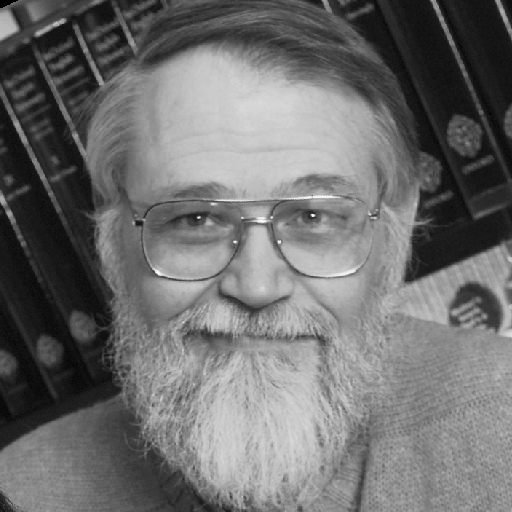
\includegraphics[width=299pt]{imagenes/brian_kernighan.png}
\end {center}
\caption{Imagen original en escala de grises de Brian Kernighan}
\label{fig:SinProm}
\end{figure}

Habiendo mostrado las diferencias entre la implementaci\'on de los filtros en
una dimensi\'on y tambi\'en habiendo portado el filtrado a trav\'es de la toma de cada
fila de la im\'agen como una se\~nal de una dimensi\'on, procedemos a mostrar
los resultados obtenidos en funci\'on de los ruidos aplicados, a diferencia de
lo realizado con una dimensi\'on, donde el foco est\'a puesto en discriminar los
resultados por tipo de filtro.

\subsubsection{Ruido gaussiano con 10 de varianza}

Este ruido es controlado y es as\'i como tambi\'en los filtros pueden volver a
una imagen muy similar a la original.

\begin{figure}[H]
    \begin{center}

    $\begin{array}{cc}
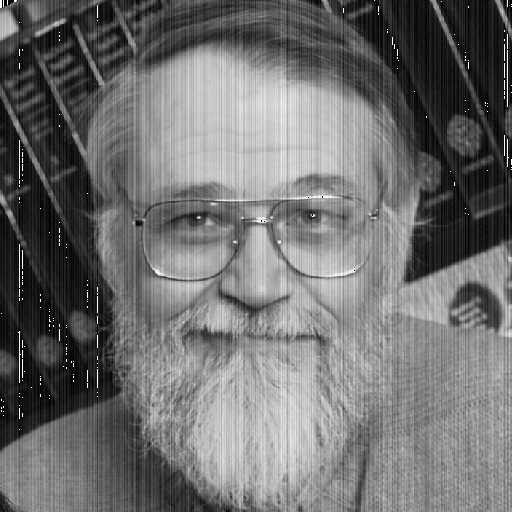
\includegraphics[width=150pt]{imagenes/kern-gauss-10-noisy.png}
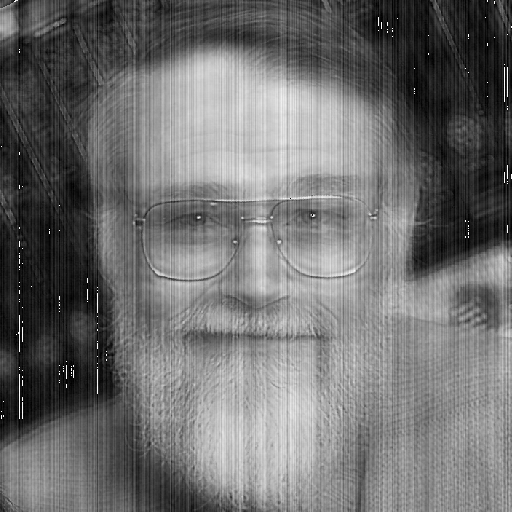
\includegraphics[width=150pt]{imagenes/kern-gauss-10-recovered-exp.png}
\end{array}$
    $\begin{array}{cc}
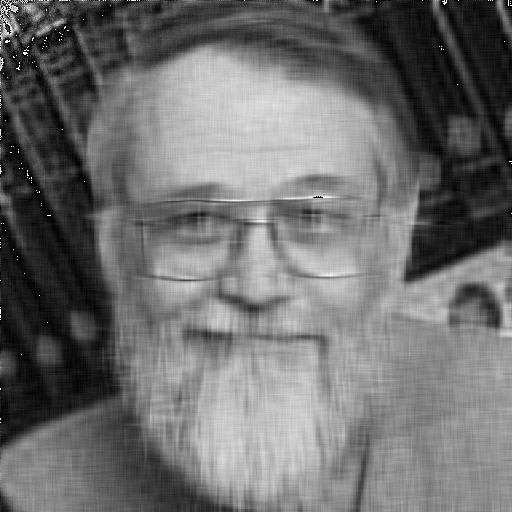
\includegraphics[width=150pt]{imagenes/kern-gauss-10-recovered-median.png}
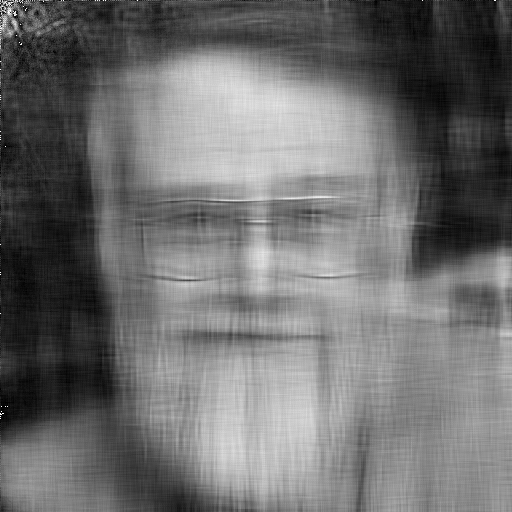
\includegraphics[width=150pt]{imagenes/kern-gauss-10-recovered-both.png}
\end{array}$
\caption{\textbf{Arriba Izquierda}: Imagen con ruido gaussiano de varianza 10, \textbf{Arriba Derecha}: Recuperada con filtro exponencial, \textbf{Abajo Izquierda}: Recuperada con filtro de la mediana, \textbf{Abajo Derecha}: Recuperada aplicando filtro exponencial y de la mediana}
 \end{center}
\label{fig:kerngauss10}
\end{figure}

\subsubsection{Ruido gaussiano con 50 de varianza}

\begin{figure}[H]

    \begin{center}
     $\begin{array}{cc}
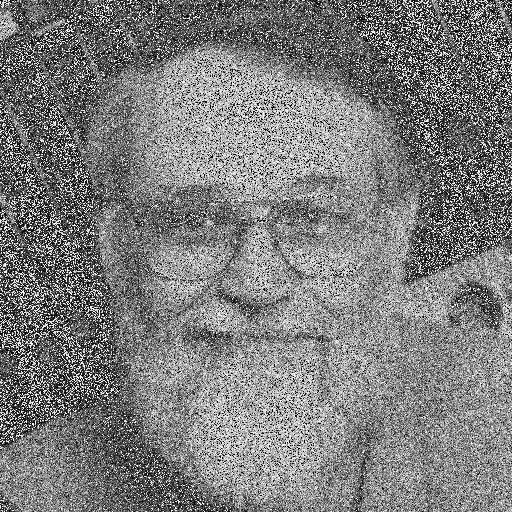
\includegraphics[width=150pt]{imagenes/kern-gauss-50-noisy.png}
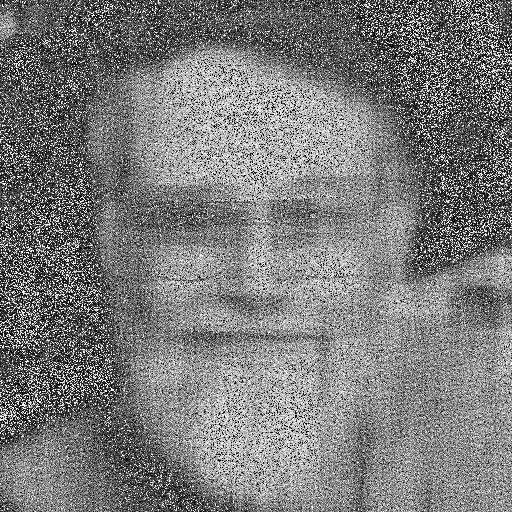
\includegraphics[width=150pt]{imagenes/kern-gauss-50-recovered-exp.png}
\end{array}$
    $\begin{array}{cc}
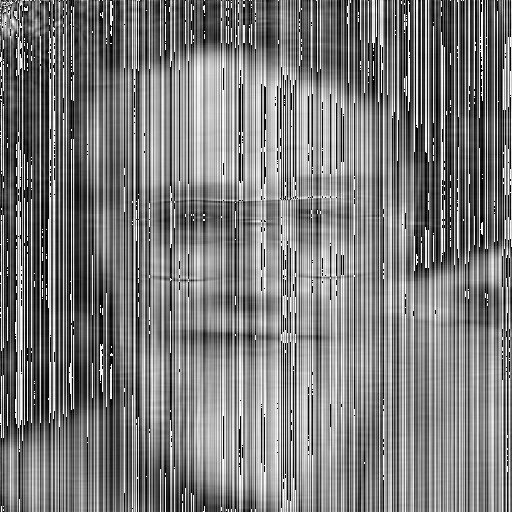
\includegraphics[width=150pt]{imagenes/kern-gauss-50-recovered-median.png}
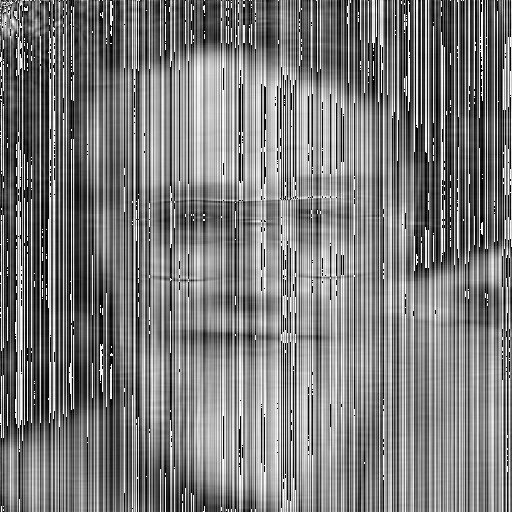
\includegraphics[width=150pt]{imagenes/kern-gauss-50-recovered-both.png}
\end{array}$
 \caption{\textbf{Arriba Izquierda}: Imagen con ruido gaussiano con varianza 50, \textbf{Arriba Derecha}: Recuperada con filtro exponencial, \textbf{Abajo Izquierda}: Recuperada con filtro de la mediana, \textbf{Abajo Derecha}: Recuperada aplicando filtro exponencial y de la mediana}
 \end{center}
\label{fig:kerngauss50}
\end{figure}


\subsubsection{Ruido impulsivo}


\begin{figure}[H]
     \begin{center}
     $\begin{array}{cc}
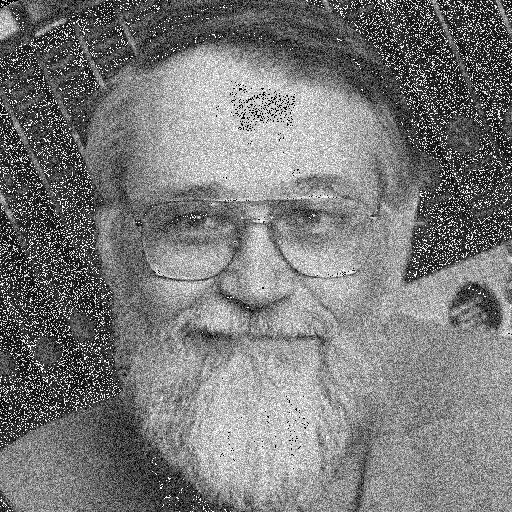
\includegraphics[width=150pt]{imagenes/kern-imp-noisy.png}
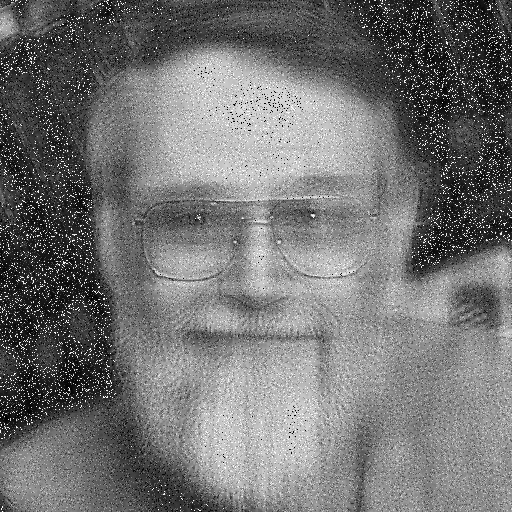
\includegraphics[width=150pt]{imagenes/kern-imp-recovered-exp.png}
\end{array}$
    $\begin{array}{cc}
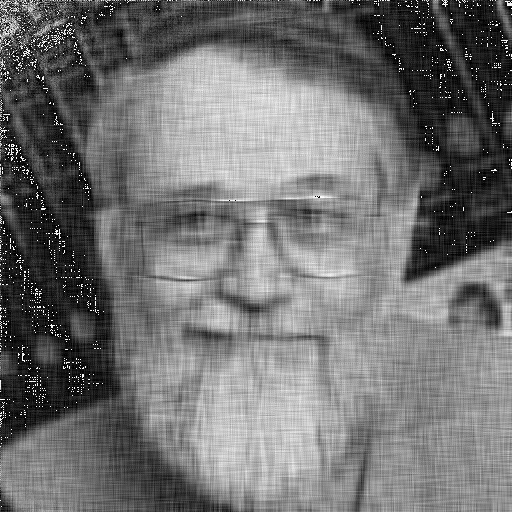
\includegraphics[width=150pt]{imagenes/kern-imp-recovered-median.png}
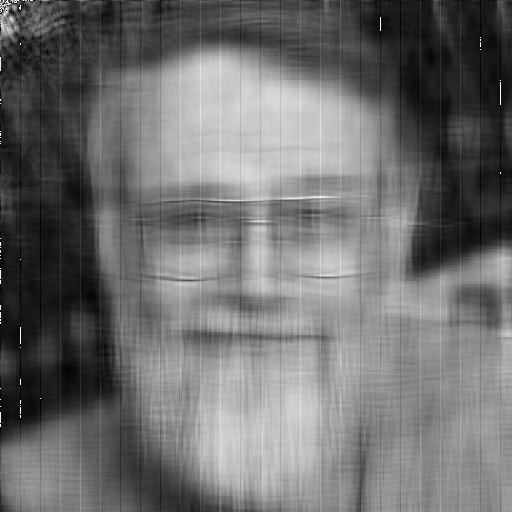
\includegraphics[width=150pt]{imagenes/kern-imp-recovered-both.png}
\end{array}$
\end{center}
 \caption{\textbf{Arriba Izquierda}: Imagen con ruido impulsivo, \textbf{Arriba Derecha}: Recuperada con filtro exponencial, \textbf{Abajo Izquierda}: Recuperada con filtro de la mediana, \textbf{Abajo Derecha}: Recuperada aplicando filtro exponencial y de la mediana}
\label{fig:kernimp}
\end{figure}

